% REP002 探索：学習ベース5手法のベースライン（親：W001。問いは未確定）
% コンパイル：uplatex を2回 → dvipdfmx（TEXINPUTS で .claude/templates/progress_report// を参照）
\documentclass[twocolumn, 10pt]{ujarticle}
\usepackage{progress_report}

\begin{document}

\reportid{REP002}
\questionid{W001}
\exploration{既存の学習ベース入札手法は，この環境でどう動くか}
\reportdate{20261008}
\summary{%
既存の学習ベース入札手法（BC，IQL，CQL，BCQ，TD3\_BC）が，このシミュレータでどう動くかを確認し，ルールベース3手法と並べたベースラインを作った。
公開データ21日分（約77GB）を取得して本家の既定設定で学習し直し，REP001と同じ48位置×4エピソードで評価したところ，全17モデル・全486 runが完走し，スコア合計はOnline LP，BCQ，BC，IQL，ABid，PIDの順であった（ABidを1.0として1.51，1.41，1.40，1.39，1.00，0.78）。
CQLとTD3\_BCは，既定の100ステップの学習では落札できずスコアがほぼ0で，20,000ステップでは他の学習ベースと同じ水準になった。
}
\beginverification

% ============================================================
\section{目的}\label{sec:e-purpose}
% ============================================================

既存の学習ベース入札手法（BC，IQL，CQL，BCQ，TD3\_BC）が，このシミュレータでどう動くかを知り，
ルールベース3手法（REP001）と並べたベースラインを作る。

% ============================================================
\section{実験}\label{sec:e-exp}
% ============================================================

\subsection{対象のアルゴリズム}\label{sec:e-algo}

5手法とも，ルールベースと同じく，入札額を「$\alpha\times$価値」で決める。$\alpha$は，過去の入札の記録（ログ）から学習した
ニューラルネットワークに，そのティックの状態を入れて出す。入力と出力は5手法で同じで，違いはログからの学ばせ方である（表\ref{tab:algo}）。

\begin{table}[H]
\centering
\caption{学習ベース5手法（上：共通の作り，下：学ばせ方の違い）}
\label{tab:algo}
\footnotesize
\begin{tabularx}{\linewidth}{@{}l>{\raggedright\arraybackslash}X@{}}
\toprule
入力（状態） & 16個の数：残り時間，残り予算の割合，入札額・落札率・価値などの平均（全体と直近），PV数。CPA制約は入らない \\
出力 & $\alpha$を1つ \\
学習の報酬 & 露出したPVの価値の和（期待購入数）。CPAのペナルティは入らない \\
\midrule
BC & ログの「この状態で，この$\alpha$」をそのまま真似る。報酬は見ない \\
IQL & その後の報酬が大きかったログの$\alpha$を，重く見て真似る \\
CQL & 報酬の見込み（Q値）が高い$\alpha$を選ぶ。ログにない$\alpha$は低く見積もる \\
BCQ & ログに出てきそうな$\alpha$の候補を作り，Q値が最大のものを選ぶ \\
TD3\_BC & Q値が高い向きに$\alpha$を動かす。ログの$\alpha$から離れると罰を受ける \\
\bottomrule
\end{tabularx}
\end{table}

\begin{figure*}[t]
\centering
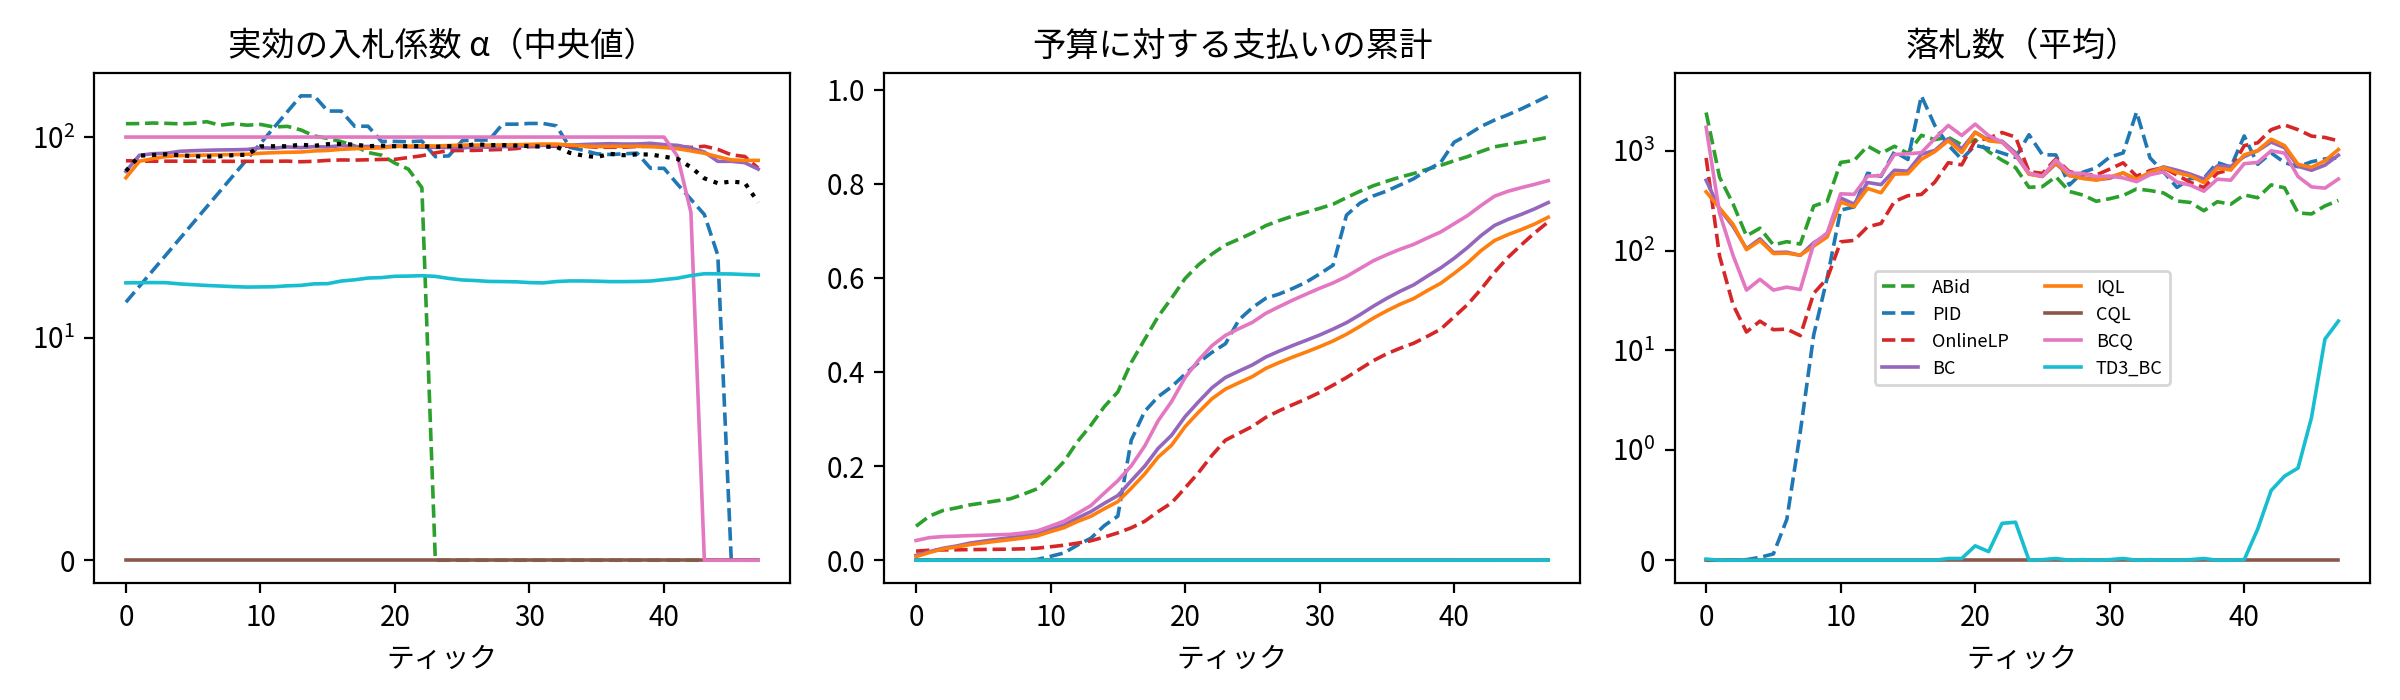
\includegraphics[width=0.86\textwidth]{fig/fig_alpha_time.png}
\caption{既定設定の8手法の時系列（192セルの中央値または平均）。破線はルールベース，点線は他47社の中央値。左：実効の入札係数$\alpha$，中：予算に対する支払いの累計，右：落札数}
\label{fig:alpha}
\end{figure*}

\subsection{実験環境}\label{sec:e-env}

公開データで学習し直した重みを，REP001と同じ方法（48社のうち1社を差し替え，scoreも同じ定義）で評価した（表\ref{tab:cond}）。
REP001はWindows，今回はLinuxで，同じ24セルを比べると1セルで購入数が違った。そのため，ルールベース3手法もこの端末で流し直した。

\begin{table}[H]
\centering
\caption{実験の条件（1 run$=$1位置$\times$4エピソード）}
\label{tab:cond}
\footnotesize
\begin{tabularx}{\linewidth}{@{}l>{\raggedright\arraybackslash}X@{}}
\toprule
学習 & 公開データ21日分（約77GB，5億行） \\
 & $\rightarrow$学習データ48,384行（広告主1社$\times$1ティック） \\
 & 本家のコードと既定の設定，乱数seed=1 \\
 & 1ステップ$=$100行で1回更新 \\
 & 既定：BC・IQL 20,000，他の3手法 100ステップ \\
\midrule
評価（固定） & シミュレータは既定の設定，乱数seed=1 \\
 & Linux，Python 3.9.16，CPU \\
\midrule
比較 & 8手法（学習ベースは既定の設定で学習した重み） \\
 & 位置48$\times$エピソード0〜3（192セル） \\
 & 計384 run \\
\midrule
学習の条件 & 位置0, 8, 16, 24, 32, 40$\times$エピソード0〜3 \\
 & (a) 乱数シード2，3で学習した重み \\
 & (b) CQL・TD3\_BCを20,000ステップ学習した重み \\
 & (c) シミュレータに同梱の学習済み重み \\
 & 計108 run \\
\bottomrule
\end{tabularx}
\end{table}

\subsection{取った特徴量}\label{sec:e-feat}

評価で記録した量はREP001と同じで，学習に関する量を足した（表\ref{tab:feat}）。

\begin{table}[H]
\centering
\caption{取った特徴量}
\label{tab:feat}
\footnotesize
\begin{tabularx}{\linewidth}{@{}l>{\raggedright\arraybackslash}X@{}}
\toprule
種類 & 記録した量 \\
\midrule
評価（REP001と同じ） & 入札の強さ，市場，予算のペース，落札の中身，CPA，位置と他社，規模 \\
学習データ & 日ごとの行数と欠損，広告主ごとの平均の$\alpha$・支払い・実績CPA \\
学習の経過 & 1ステップごとの損失，所要時間，重みのハッシュ \\
重みの出どころ & 結果ごとに，手法・ステップ数・乱数シード \\
\bottomrule
\end{tabularx}
\end{table}

% ============================================================
\section{結果}\label{sec:e-result}
% ============================================================

\textbf{データと学習}　公開データ21日分（5億行）を取得でき，学習データ48,384行を作れた。欠損は，3日分の終盤にある入札額の62,153行だけで，その行は落札していなかった。
17モデルがすべて学習でき，損失は最後まで有限であった。既定設定の5モデルは，学習し直すと同じ重みになった。
学習の所要時間（CPU）は，既定設定で13〜93秒，20,000ステップのCQLが429秒，TD3\_BCが771秒であった。
BCQは1ステップ約0.57秒で，20,000ステップは約3時間の見込みのため，事前に決めた打ち切りに従って流さなかった。

\textbf{評価の動作と規模感}　486 runがすべて完走した。1 runは7〜8並列で152〜176秒，最大メモリは約2.9GBであった。
\texttt{bidding()}1回の平均は，BC・IQL・CQL・TD3\_BCが約12ms，BCQが48ms（最大240ms），ルールベースは0.13〜1.6msであった。

\textbf{8手法の比較}　表\ref{tab:cmp}と図\ref{fig:scores}のとおり，score合計は，Online LP，BCQ，BC，IQL，ABid，PID，TD3\_BC，CQLの順であった。
BCQ・BC・IQLは，Online LPの0.92〜0.94倍であった。
既定設定のCQLは，全ティックで$\alpha$が0で，1度も落札しなかった。TD3\_BCは$\alpha$が約19で（他47社の中央値は約83），192セルの購入数の合計は8であった（図\ref{fig:alpha}）。
BCQの$\alpha$の中央値は，ティック0〜41で100のまま変わらなかった。
セル単位でOnline LPを上回った割合は，BC 0.48，IQL 0.47，BCQ 0.45であった。
カテゴリ別の合計が最大だった手法は，Online LPが3つ，IQL，BCQ，BCが1つずつであった。
ルールベース3手法の値は，REP001（Windows）とほぼ同じであった（Online LP 1.49と1.51，PID 0.78と0.78）。
論文の図10（目視の概算，ABidを1.0）はOnline LP 6.5〜7，IQL 2.6〜3，BC 2.3〜2.5で，倍率は本結果と一致しない（原因は未確認）。

\begin{table}[H]
\centering
\caption{既定設定の8手法（48位置×4エピソード，192セル）}
\label{tab:cmp}
\footnotesize\setlength{\tabcolsep}{3pt}
\begin{tabularx}{\linewidth}{@{}Xrrrrr@{}}
\toprule
 & score合計 & ABid比 & 平均報酬 & 罰の割合 & 消化率 \\
\midrule
Online LP & 0.247 & 1.51 & 28.8 & 0.39 & 0.75 \\
BCQ & 0.232 & 1.41 & 28.9 & 0.45 & 0.83 \\
BC & 0.229 & 1.40 & 28.4 & 0.44 & 0.77 \\
IQL & 0.228 & 1.39 & 27.9 & 0.44 & 0.74 \\
ABid & 0.164 & 1.00 & 25.8 & 0.85 & 0.93 \\
PID & 0.129 & 0.78 & 24.4 & 0.82 & 0.99 \\
TD3\_BC & 0.0004 & 0.002 & 0.04 & 0.21 & 0.00 \\
CQL & 0 & 0 & 0 & 0 & 0.00 \\
\bottomrule
\end{tabularx}
\par\smallskip
\raggedright score合計は20000で割った値。平均報酬はペナルティ前の購入数。罰の割合はCPA超過のペナルティが掛かったセルの割合。消化率は予算消化率の平均。
\end{table}

\begin{figure}[H]
\centering
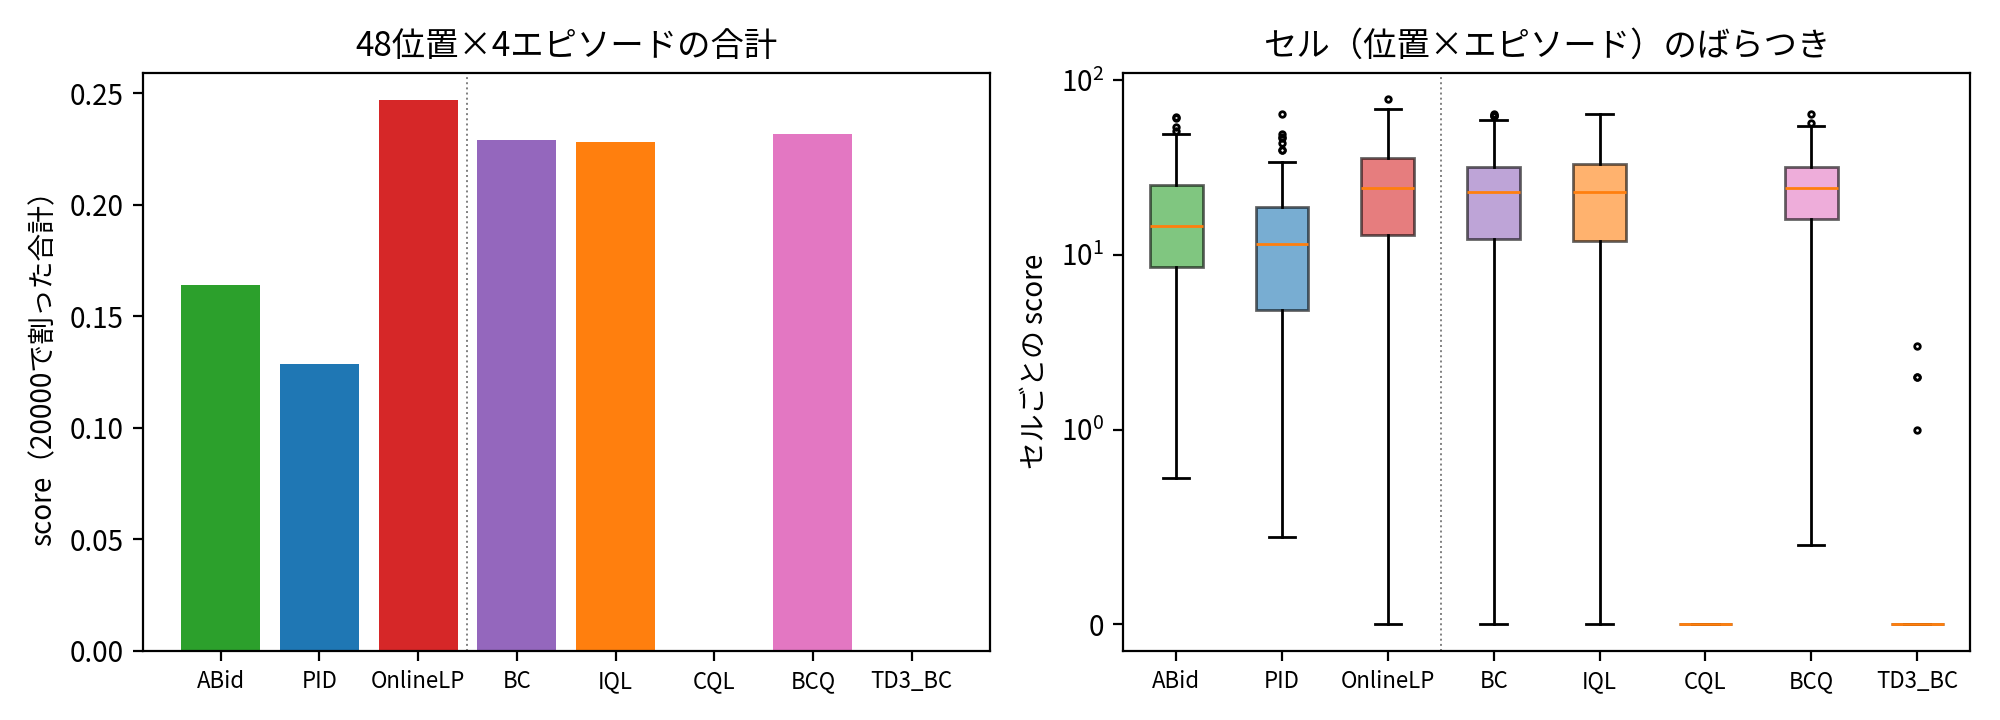
\includegraphics[width=\linewidth]{fig/fig_scores.png}
\caption{8手法のスコア。左：合計，右：セルごとの分布（symlog軸）}
\label{fig:scores}
\end{figure}

\textbf{学習の条件}　表\ref{tab:var}と図\ref{fig:var}は，6位置×4エピソード（24セル）の平均scoreである。同じ24セルで，Online LPは23.4，PIDは15.5，ABidは12.0であった。
CQLとTD3\_BCは，既定の100ステップでは3つのseedすべてで0で，20,000ステップでは18.6と21.5になった。
BCQ（100ステップ）は，seed 1・2が21.7，seed 3が0であった。BCとIQLは，seedを変えても既定の0.96〜1.03倍に収まった。
同梱の重みは，BCとIQLでは自前の重みの0.81倍・0.84倍，BCQでは1.06倍であった。

\begin{table}[H]
\centering
\caption{学習の条件を変えたときの平均score（24セル）}
\label{tab:var}
\footnotesize\setlength{\tabcolsep}{3pt}
\begin{tabularx}{\linewidth}{@{}Xrrrrr@{}}
\toprule
 & seed 1 & seed 2 & seed 3 & 2万ステップ & 同梱 \\
\midrule
BC & 20.5 & 21.2 & 20.4 & （既定） & 16.6 \\
IQL & 21.3 & 20.9 & 20.4 & （既定） & 17.8 \\
CQL & 0 & 0 & 0 & 18.6 & 17.9 \\
BCQ & 21.7 & 21.7 & 0 & 未実施 & 23.0 \\
TD3\_BC & 0 & 0 & 0 & 21.5 & 19.5 \\
\bottomrule
\end{tabularx}
\par\smallskip
\raggedright seed 1〜3は既定のステップ数（BC・IQLは2万，他は100）。
\end{table}

\begin{figure}[H]
\centering
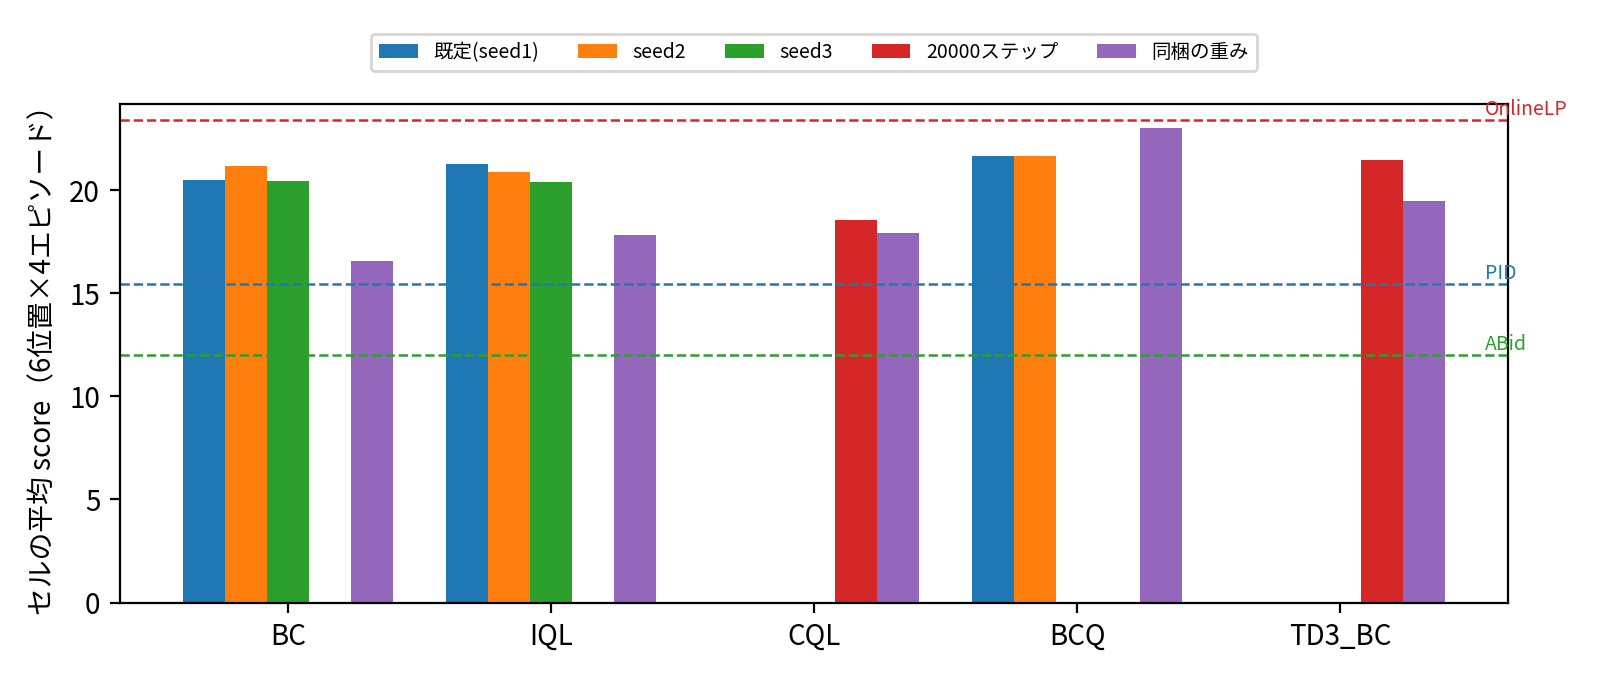
\includegraphics[width=\linewidth]{fig/fig_variants.png}
\caption{学習の条件を変えたときの平均score（24セル）。破線はルールベース3手法}
\label{fig:var}
\end{figure}

\textbf{特徴量}　\texttt{episodes}（1,944行），\texttt{ticks}（93,312行），\texttt{agents}（93,312行）の全数値列に，NaN・無限大はなかった。

以上より，実験の前に決めた達成条件（REP002.md）を満たし，探索の目的は\textbf{達成}した。
ただし，BCQの20,000ステップは打ち切りの決まりで流しておらず，既定の成績が0のCQLとTD3\_BCは，既定に対する比ではなく成績そのものを記録した。

\end{document}
